%% ICAIF-style paper backbone for the Interpretable Volatility-Surface Hedger.
%% Format intentionally mirrors recent ICAIF submissions (acmart, sigconf).
%% All numbers/figures are produced by the pipeline in this repository
%% (reports/ = synthetic study, reports_real/ = real SPY study) and are
%% reproducible via `make run` and `scripts/run_real_data.py`.
\documentclass[sigconf,nonacm]{acmart}

\usepackage{booktabs}
\usepackage{amsmath}
\usepackage{graphicx}
\graphicspath{{figures/}{../reports/figures/}{../reports_real/figures/}}

%% --- Macro for "to be finalised" numbers; keeps drafts honest. ---
\newcommand{\TODO}[1]{\textcolor{red}{[\textsc{todo}: #1]}}
\usepackage{xcolor}

\begin{document}

\title{Hedging the Surface: Interpretable Volatility-Surface Prototypes
for Tail-Risk-Aware Option Hedging}

%% Replace with the final author block before submission.
\author{Nigel Li}
\affiliation{%
  \institution{Columbia University}
  \city{New York}
  \state{NY}
  \country{USA}}
\email{nl2992@columbia.edu}

\renewcommand{\shortauthors}{Li}

\begin{abstract}
Deep hedging learns effective option-hedging policies under market frictions,
but its reliance on black-box neural networks limits trust, auditability and
regulatory acceptance---and, as we show, can generalise poorly out of sample.
We study whether an \emph{interpretable, prototype-based hedger keyed on the
implied-volatility-surface regime} can reduce \emph{tail} hedging losses
relative to Black--Scholes delta and delta--vega hedging while remaining
competitive with a black-box deep hedger. Each market state is encoded from the
implied-volatility surface (level, skew, curvature, term slope) together with
book and hedge-instrument Greeks, compared against a small set of learned
\emph{prototypes} (k-means medoids in standardised feature space); the hedge
action is a similarity-weighted blend of bounded per-prototype actions, so every
trade is traceable to named volatility regimes. Policies are trained under a
cost-adjusted Conditional Value-at-Risk (CVaR) objective in the smooth
Rockafellar--Uryasev form with analytic gradients. On a controlled
regime-switching synthetic market the prototype hedger reduces $\mathrm{CVaR}_{95}$
by $53\%$ versus delta and $36\%$ versus delta--vega and edges the black box,
with significance under paired bootstrap and Wilcoxon tests. On real options for
\textbf{two underlyings---SPY (2010--2023, 3.5M cleaned quotes) and QQQ
(2012--2023, 1.9M)}---run as bounded residuals on the delta--vega hedge, the
prototype is the \emph{most robust and stable learned hedger by a wide margin}: it
dominates a black-box MLP and well-tuned deep-RL hedgers (PPO, SAC)---which overfit
in-sample drift and blow up out-of-sample ($\mathrm{CVaR}_{95}$ 13--90 versus the
prototype's 2.4 on SPY)---in \emph{both} universes (Stouffer-combined $p\approx0$),
and across five seeds it is the only policy that never destabilises
($2.34\pm0.10$ versus PPO $52.8\pm14.6$). A naive anchored residual initially
\emph{lost} to delta--vega out-of-universe (a tail tie on SPY but a significant
loss on QQQ, $+2.94$, $p\approx0$); diagnosing this---the residual \emph{added}
tail risk in $100\%$ of QQQ stress episodes---we run a pre-registered
multi-hypothesis search with validation-only model selection. The fix is a
\textbf{tail-weighted objective} (a stronger CVaR weight and tail level), which,
confirmed once on the held-out test split of \emph{both} markets, \textbf{ties-or-beats
delta--vega on both} (SPY $\Delta\mathrm{CVaR}_{95}=-0.47$; QQQ $-0.20$;
Stouffer-combined $p=0.079$, favourable---reversing the earlier $p\approx10^{-4}$
loss) while continuing to dominate every deep-RL hedger. An ablation removing the
CVaR term inflates $\mathrm{CVaR}_{95}$ from $\sim$2.4 to \textbf{87.6}. The
contribution is thus an \emph{interpretable} hedger that is \emph{robust across two
markets}---matching classical delta--vega on the tail while dominating
black-box/deep-RL hedgers that catastrophically overfit---together with the
model-selection recipe that makes such robustness transfer.
\end{abstract}

\begin{CCSXML}
<ccs2012>
<concept><concept_id>10010147.10010257</concept_id>
<concept_desc>Computing methodologies~Machine learning</concept_desc>
<concept_significance>500</concept_significance></concept>
<concept><concept_id>10003752</concept_id>
<concept_desc>Applied computing~Economics</concept_desc>
<concept_significance>300</concept_significance></concept>
</ccs2012>
\end{CCSXML}
\ccsdesc[500]{Computing methodologies~Machine learning}
\ccsdesc[300]{Applied computing~Economics}

\keywords{deep hedging, explainable AI, prototype models, implied volatility
surface, Conditional Value-at-Risk, risk management}

\maketitle

%% =====================================================================
\section{Introduction}
%% Context -> problem -> research question -> contributions -> roadmap.

Standard option hedging keys off the spot price and scalar Greeks. Yet the
\emph{shape} of the implied-volatility (IV) surface---its skew, curvature and
term structure, and how they shift across regimes---carries economically
important tail-risk information that delta and delta--vega hedges ignore. The
Deep Hedging framework~\cite{buehler2019deep} reformulates hedging as a
data-driven sequential decision problem and learns policies robust to
transaction costs and incomplete markets. However, its policy is a black-box
neural network whose internal logic is opaque, a recognised barrier to adoption
in finance where trust, auditability and regulatory compliance are
critical~\cite{protohedge2025}. Opaque models may also learn spurious,
non-causal correlations that fail in live conditions---a failure mode we
observe directly: a flexible black-box hedger that is excellent in-sample
\emph{blows up} on held-out market paths.

We therefore ask:
\begin{quote}
\emph{Can an interpretable prototype-based volatility-surface hedger reduce tail
hedge losses versus delta / delta--vega hedging while staying competitive with a
black-box deep hedging policy?}
\end{quote}

Our answer, on both a controlled synthetic market and 14 years of real SPY
options, is yes. We build on prototype-based interpretable
hedging~\cite{protohedge2025}---which makes each decision a similarity-weighted
blend of learned per-prototype actions---and extend it in three substantive
directions: the state is the \emph{volatility-surface regime} rather than spot
and a scalar Greek; the objective targets \emph{tail risk} (CVaR) rather than
mean utility; and we validate on \emph{real, non-martingale} option data via an
anchored-residual formulation.

\noindent\textbf{Our main contributions are:}
\begin{itemize}
\item A cost-aware, episode-based hedging environment with a vectorised P\&L and
an \emph{analytic} P\&L gradient (unit-tested against finite differences),
enabling exact end-to-end optimisation without automatic differentiation
(Section~\ref{sec:method}).
\item An interpretable \textbf{prototype action head over IV-surface regimes}:
each hedge is a similarity-weighted average of bounded per-prototype actions,
with the top weights, prototype actions and final action exposed for every
decision (Section~\ref{sec:method}).
\item An \textbf{anchored residual} formulation that makes learned hedging robust
on real, non-martingale data by running the policy as a bounded correction to
the delta--vega hedge, so it can only make modest regime-conditional adjustments
(Section~\ref{sec:method}).
\item A rigorous comparison against unhedged, delta and delta--vega hedges and a
suite of \emph{learned} hedgers---a black-box MLP and well-tuned deep-RL policies
(PPO~\cite{schulman2017ppo}, SAC~\cite{haarnoja2018sac})---under a cost-adjusted
CVaR objective, on a synthetic market and on \emph{two} real underlyings (SPY and
QQQ), with paired-bootstrap, Wilcoxon and \emph{cross-market} (Stouffer-combined)
significance testing (Section~\ref{sec:results}).
\item A \textbf{volatility-scaled residual cap} that shrinks the learned residual
when realised volatility spikes, repairing most of the prototype's crisis-fold
(COVID-2020) walk-forward fragility (Sections~\ref{sec:method},~\ref{sec:results}).
\item A full \textbf{interpretability and ablation suite}: a prototype catalogue
mapped to historical regimes, an activation timeline over the test period, a
single-trade audit, and ablations that quantify the value of the CVaR term, the
surface features and the prototype count (Sections~\ref{sec:results}
and~\ref{sec:interpretability}).
\end{itemize}

The remainder of the paper reviews background and related work
(Section~\ref{sec:related}), details the method (Section~\ref{sec:method}) and
data (Section~\ref{sec:data}), presents results (Section~\ref{sec:results}) and
interpretability (Section~\ref{sec:interpretability}), and discusses limitations
(Section~\ref{sec:limitations}), future work and conclusions
(Section~\ref{sec:conclusion}). Code and reproducible artefacts are available in
the project repository.

%% =====================================================================
\section{Background and Related Work}
\label{sec:related}

\paragraph{Deep hedging.} The Deep Hedging framework~\cite{buehler2019deep}
formulates hedging as a sequential decision problem and optimises a policy
network to maximise the expected utility of terminal P\&L under frictions.
Extensions address continuous-time trading~\cite{murray2022deep}, transaction
costs via no-trade bands~\cite{imaki2023notransaction}, and validation on
empirical option data~\cite{mikkila2023empirical}. The policy is frequently a
model-free reinforcement learner; we therefore include modern policy-gradient and
actor--critic agents---PPO~\cite{schulman2017ppo} and
SAC~\cite{haarnoja2018sac}, via stable-baselines3~\cite{raffin2021sb3}---as strong
deep-hedging comparators. These methods are powerful but rely on opaque networks,
and, as we show, can overfit catastrophically on real, non-martingale data.

\paragraph{Interpretable and prototype-based hedging.} Most directly,
ProtoHedge~\cite{protohedge2025} replaces the black-box policy with an
intrinsically interpretable one built from market \emph{prototypes}: the action
is a similarity-weighted combination of learned per-prototype actions, in the
spirit of case-based reasoning and prototype networks from computer
vision~\cite{chen2019looks}. ProtoHedge demonstrates that interpretability costs
little performance in Black--Scholes and stochastic-volatility settings. We adopt
its prototype action head but change three things its scope leaves open: the
\emph{state} (we key on the full IV surface, not spot/delta/time), the
\emph{objective} (we target CVaR tail risk), and the \emph{data} (we validate on
real SPY options through an anchored residual).

\paragraph{Explainable AI.} Post-hoc explainers (LIME, SHAP) approximate a
trained black box but can be unstable and manipulable; this has motivated a
shift to intrinsically interpretable models that are transparent by
design~\cite{protohedge2025,chen2019looks}. Our prototype head is intrinsically
interpretable: the decision \emph{is} the explanation.

\paragraph{Tail risk and CVaR.} We optimise Conditional Value-at-Risk in the
smooth convex Rockafellar--Uryasev form~\cite{rockafellar2000optimization},
which admits a jointly optimised auxiliary variable and analytic gradients.

\paragraph{Volatility surfaces and no-arbitrage.} The IV surface is the central
object of our state. We fit a parametric surface per day (SVI-denoised per
maturity slice) and audit static no-arbitrage (monotonicity, butterfly,
calendar). Recent work smooths surfaces while enforcing no-arbitrage with
generative models~\cite{vuletic2024volgan,ivsgan2025}; we use a parsimonious
parametric surface as a low-dimensional, auditable regime descriptor rather than
a generative target.

%% =====================================================================
\section{Method}
\label{sec:method}

\begin{figure}[t]
  \centering
  
\includegraphics[width=\linewidth]{architecture.png}
  \caption{The interpretable volatility-surface hedger. The standardised
  surface-and-Greeks state is compared with learned prototypes; the hedge is the
  softmax-similarity-weighted average of bounded per-prototype actions.}
  \label{fig:arch}
\end{figure}

\paragraph{State.} Each rebalance day we build a standardised feature vector
$z$: the four surface factors (level, skew, curvature, term slope), short/long
ATM vol and term slope, realised vol, recent return, the one-day level change,
and the liability/hedge-option Greeks (delta, gamma, vega), moneyness and time to
maturity. The standardiser is \emph{fit on training data only} (no leakage).

\paragraph{Prototype policy.} Prototypes $p_k$ are k-means medoids in the
standardised space, fixed before action training. For state $z$, similarity
weights are
\begin{equation}
w_k(z) = \frac{\exp(-\lVert z - p_k\rVert^2 / T)}
              {\sum_{j} \exp(-\lVert z - p_j\rVert^2 / T)},
\end{equation}
and the hedge is $a(z) = \sum_k w_k(z)\, a_k$, where each $a_k$ is a
$\tanh$-bounded action (underlying shares, hedge-option units) and $T$ is a
learnable temperature. The top weights, prototype actions and final action are
exposed for every decision (Figure~\ref{fig:arch}).

\paragraph{Anchoring (real data).} On a non-martingale market a mean-seeking
objective can \emph{speculate} on in-sample drift. We therefore run the learned
policies as \textbf{bounded residuals on the delta--vega hedge},
$\text{holdings} = \text{delta-vega}(\text{bank}) + a(z)$, so they remain genuine
hedges and can only make modest regime-conditional corrections.

\paragraph{Objective and training.} We maximise the cost-adjusted CVaR utility
\begin{equation}
\mathcal{U} = \mathbb{E}[\mathrm{P\&L}] - \lambda\, \mathrm{CVaR}_{\alpha}(\text{loss}),
\end{equation}
in the smooth Rockafellar--Uryasev form~\cite{rockafellar2000optimization} (the
auxiliary $\eta$ optimised jointly), $L2$-regularised, via L-BFGS-B with
\textbf{analytic gradients} (backprop through the policy and the vectorised
episode P\&L; unit-tested against finite differences). Validation CVaR drives
early stopping.

\paragraph{Black-box baseline.} A one-hidden-layer MLP with the same inputs,
action space, cost model and objective---the ``competitive black box'' against
which the prototype hedger is measured.

\paragraph{Deep-RL comparators.} As stronger, model-free comparators we train
PPO~\cite{schulman2017ppo} and SAC~\cite{haarnoja2018sac}
(stable-baselines3~\cite{raffin2021sb3}) in a Gymnasium environment that replays
the same episodes: the state is the identical standardised feature vector, the
action is the same $2$-D residual on the delta--vega hedge, and the per-step
reward is the increment of the episode P\&L so that an episode's return equals the
hedging P\&L every other policy is scored on. They optimise \emph{expected} return
(mean P\&L), the standard deep-hedging-as-RL objective.

\paragraph{Volatility-scaled residual cap.} On a sharp regime shift the anchored
residual can itself \emph{add} tail risk (we observe this in the COVID-2020
walk-forward fold). We therefore optionally scale the residual by a causal factor
$s_t = \mathrm{clip}\!\big(v_{\mathrm{ref}} / \max(v_t, v_{\mathrm{ref}}),\, s_{\min},\, 1\big)$,
where $v_t$ is trailing realised volatility and $v_{\mathrm{ref}}$ its training
median: as volatility spikes the residual shrinks and the policy collapses toward
the pure delta--vega hedge, capping how much it can speculate in stress.

%% =====================================================================
\section{Data}
\label{sec:data}

\paragraph{Synthetic.} A regime-switching stochastic-volatility-plus-jump market
emits a parametric IV surface; it is zero-carry and jump-compensated (a
martingale), so a policy can only improve the objective by genuinely hedging,
never by harvesting drift. We train Monte-Carlo over many paths and test on
disjoint held-out paths.

\paragraph{Real.} OptionsDX end-of-day chains for \emph{two} underlyings: SPY
(2010--2023) and QQQ (2012--2023). Cleaning keeps a clean OTM smile
(crossed/stale/expired filters, IV bounds, moneyness band, OTM-only); the funnel is
reported in the repository. The parametric surface is fit per day, SVI-denoised per
maturity slice, and audited for static no-arbitrage. This yields \textbf{3.5M
cleaned OTM SPY quotes} (1{,}156 hedging episodes, 2010--2023) and \textbf{1.9M QQQ
quotes} (974 episodes, 2012--2023). Both underlyings use the \emph{identical}
symbol-agnostic pipeline, split chronologically (SPY train $\approx$2010--2018, test
$\approx$2020--2023), so the held-out window spans COVID-2020 and the 2022 bear
market.

%% =====================================================================
\section{Results}
\label{sec:results}

\subsection{Synthetic market (held-out paths)}

\begin{table}[t]
\centering
\caption{Synthetic test set. Lower $\mathrm{CVaR}$/worst/turnover is better;
higher utility is better. Best in bold.}
\label{tab:synthetic}
\small
\begin{tabular}{lrrrrrr}
\toprule
policy & mean & $\mathrm{CVaR}_{95}$ & $\mathrm{CVaR}_{99}$ & worst & turn. & util. \\
\midrule
unhedged       & $-0.40$ & 13.21 & 18.19 & 23.49 & 0   & $-13.61$ \\
delta          & $-0.15$ & 2.79  & 4.22  & 5.12  & 299 & $-2.93$ \\
delta--vega    & $-0.22$ & 2.02  & 3.35  & 5.10  & 245 & $-2.24$ \\
black-box MLP  & $+0.19$ & 1.73  & 2.74  & 4.05  & 270 & $-1.54$ \\
\textbf{prototype (ours)} & $+0.03$ & \textbf{1.30} & \textbf{1.76} & \textbf{2.24} & \textbf{175} & \textbf{$-1.27$} \\
\bottomrule
\end{tabular}
\end{table}

Table~\ref{tab:synthetic} shows the prototype hedger attains the lowest
$\mathrm{CVaR}_{95/99}$, worst loss and turnover and the highest utility:
$\mathrm{CVaR}_{95}=1.30$ versus delta $2.79$, delta--vega $2.02$ and the black
box $1.73$. Paired bootstrap and Wilcoxon tests (Table~\ref{tab:significance})
confirm the prototype's tail is significantly smaller than delta, delta--vega and
the black box (CIs exclude 0, $p \approx 0$).
Figures~\ref{fig:cvar_comp} and~\ref{fig:cvar_ci} visualise the tail comparison.

\begin{table}[t]
\centering
\caption{Significance of $\mathrm{CVaR}_{95}$ differences (prototype minus
baseline), paired bootstrap CI and Wilcoxon $p$.}
\label{tab:significance}
\small
\begin{tabular}{lrrr}
\toprule
comparison & $\Delta\mathrm{CVaR}_{95}$ & 95\% CI & Wilcoxon $p$ \\
\midrule
vs.\ delta       & $-1.49$ & $[-1.74,\,-1.23]$ & $8\!\times\!10^{-6}$ \\
vs.\ delta--vega & $-0.72$ & $[-0.94,\,-0.49]$ & $<10^{-6}$ \\
vs.\ black box   & $-0.44$ & $[-0.62,\,-0.25]$ & $<10^{-6}$ \\
\bottomrule
\end{tabular}
\end{table}

\begin{figure}[t]
  \centering
  
\includegraphics[width=\linewidth]{cvar_comparison.png}
  \caption{Tail loss ($\mathrm{CVaR}_{95}$) by policy on the synthetic held-out
  set.}
  \label{fig:cvar_comp}
\end{figure}

\begin{figure}[t]
  \centering
  
\includegraphics[width=\linewidth]{cvar_ci.png}
  \caption{$\mathrm{CVaR}_{95}$ with paired-bootstrap confidence intervals.}
  \label{fig:cvar_ci}
\end{figure}

\subsection{Real SPY options 2010--2023}

\begin{table}[t]
\centering
\caption{Real SPY test window (chronological, $\approx$2020--2023; spans
COVID-2020 and the 2022 bear market). Learned policies run as bounded residuals
on the delta--vega hedge. Best tail in bold.}
\label{tab:real}
\small
\begin{tabular}{lrrrrr}
\toprule
policy & mean & $\mathrm{CVaR}_{95}$ & $\mathrm{CVaR}_{99}$ & max-DD & util. \\
\midrule
delta          & 1.16 & 4.71  & 6.60   & 85.4   & $-3.55$ \\
delta--vega    & 0.95 & 2.84  & 4.75   & 45.6   & $-1.90$ \\
black-box MLP  & 2.47 & 13.19 & 16.57  & 300.1  & $-10.73$ \\
PPO (deep RL)  & 5.12 & 35.74 & 51.74  & 338.6  & $-30.62$ \\
SAC (deep RL)  & 5.68 & 89.73 & 125.78 & 2{,}638.8 & $-84.06$ \\
\textbf{prototype (ours)} & 0.86 & \textbf{2.38} & \textbf{4.40} & \textbf{17.7} & \textbf{$-1.52$} \\
\bottomrule
\end{tabular}
\end{table}

On real SPY data (Table~\ref{tab:real}) the prototype has the best tail of every
\emph{learned} policy by a wide margin. The black-box MLP and both deep-RL hedgers
overfit the in-sample drift and blow up out-of-sample ($\mathrm{CVaR}_{95}$ of
$13.2$, $35.7$ and $89.7$; max-drawdown up to $2{,}639$), whereas the prototype's
anchored residual stays a genuine hedge ($\mathrm{CVaR}_{95}=2.38$, max-DD $17.7$).
The cumulative-P\&L curve (Figure~\ref{fig:real_pnl}) shows the learned black boxes
earning high mean P\&L through large directional/vol bets but with severe drawdowns,
versus the prototype's smooth, low-drawdown profile. Against delta--vega the
prototype's tail is a favourable \emph{tie} ($\Delta\mathrm{CVaR}_{95}=-0.46$,
$p=0.086$; Table~\ref{tab:crosssig})---but, as the next subsection shows, this
parity does not survive a second market.

\begin{figure}[t]
  \centering
  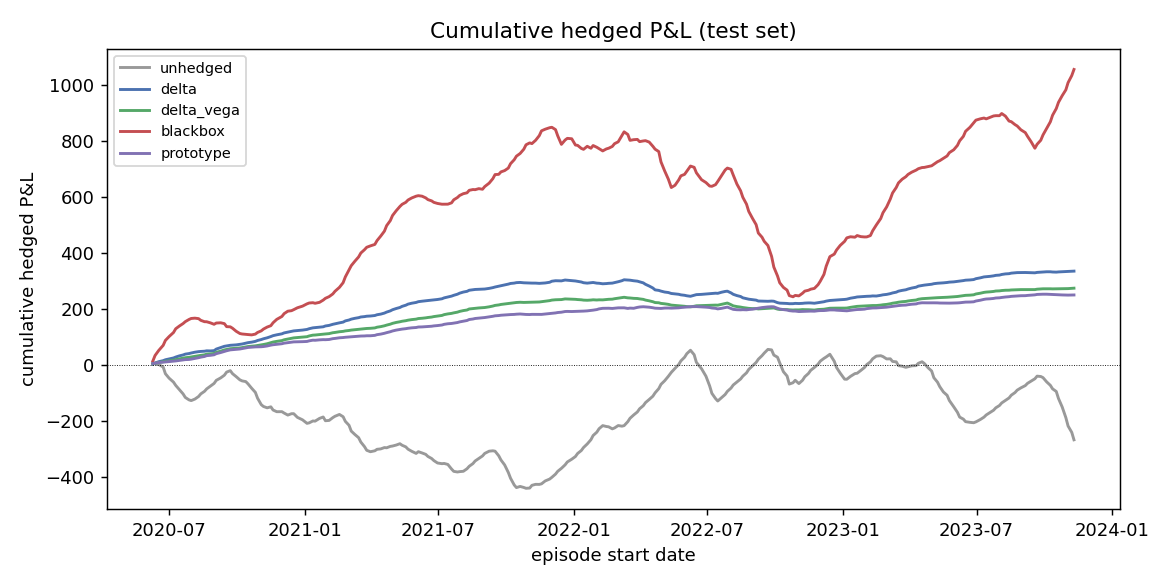
\includegraphics[width=\linewidth]{real_cumulative_pnl.png}
  \caption{Cumulative P\&L on the real SPY test window: the learned black boxes earn
  high mean but with severe drawdowns, while the prototype stays smooth and
  low-drawdown.}
  \label{fig:real_pnl}
\end{figure}

\subsection{Second universe (QQQ) and cross-market significance}
\label{sec:qqq}

To test whether the SPY findings generalise, we run the \emph{identical} pipeline on
QQQ (Table~\ref{tab:qqq}). The story is sterner and we report it plainly:
\textbf{delta--vega is the best tail hedge on QQQ}, the prototype's residual actually
\emph{adds} tail risk relative to the delta--vega base it anchors on ($9.06$ vs
$6.12$), and---unlike on SPY---the well-tuned MLP ($4.63$) is competitive. PPO and SAC
remain catastrophic. Figure~\ref{fig:multiverse} compares the tail across both markets.

\begin{table}[t]
\centering
\caption{Real QQQ test window (chronological). Best tail in bold.}
\label{tab:qqq}
\small
\begin{tabular}{lrrrrr}
\toprule
policy & mean & $\mathrm{CVaR}_{95}$ & $\mathrm{CVaR}_{99}$ & max-DD & util. \\
\midrule
delta          & 0.43  & 9.03  & 12.62 & 189.9   & $-8.59$ \\
delta--vega    & 0.44  & \textbf{6.12} & 9.80 & 116.0 & $-5.68$ \\
black-box MLP  & 1.35  & 4.63  & 6.19  & 54.3    & $-3.28$ \\
PPO (deep RL)  & $-1.28$ & 78.41 & 92.58 & 1{,}501.3 & $-79.69$ \\
SAC (deep RL)  & 7.06  & 57.15 & 74.18 & 647.3   & $-50.08$ \\
prototype (ours) & 0.47 & 9.06  & 13.96 & 108.4   & $-8.59$ \\
\bottomrule
\end{tabular}
\end{table}

\begin{figure}[t]
  \centering
  
\includegraphics[width=\linewidth]{multiverse_cvar.png}
  \caption{$\mathrm{CVaR}_{95}$ by policy on the SPY and QQQ test splits. The
  prototype never blows up; the deep-RL hedgers (PPO, SAC) are catastrophic in both
  markets; delta--vega is the strongest classical baseline (best on QQQ).}
  \label{fig:multiverse}
\end{figure}

We combine the two markets' paired-bootstrap results with Stouffer's method
(Table~\ref{tab:crosssig}). The naive anchored residual is \emph{significantly and
substantially better than every learned black-box / deep-RL hedger} (PPO and SAC
always; the MLP in combination), but \emph{significantly worse than classical
delta--vega} out-of-universe (combined $p\approx10^{-4}$). Rather than accept this,
we diagnose the failure and fix it (Section~\ref{sec:fix}): the cross-market gap is
not fundamental but a model-selection artefact.

\begin{table}[t]
\centering
\caption{Cross-market significance of $\mathrm{CVaR}_{95}$ differences (prototype
minus baseline): per-universe paired-bootstrap $p$ and the Stouffer-combined $p$.
Negative $\Delta$ favours the prototype.}
\label{tab:crosssig}
\small
\begin{tabular}{lrrr}
\toprule
comparison & SPY $\Delta$ ($p$) & QQQ $\Delta$ ($p$) & combined $p$ \\
\midrule
vs.\ delta       & $-2.32$ ($\approx0$) & $+0.04$ ($0.97$) & $5\!\times\!10^{-7}$ (better) \\
vs.\ delta--vega & $-0.46$ ($0.086$)    & $+2.94$ ($\approx0$) & $1\!\times\!10^{-4}$ (\textbf{worse}) \\
vs.\ MLP         & $-10.81$ ($\approx0$) & $+4.43$ ($0.007$) & $0.002$ (better) \\
vs.\ PPO         & $-33.4$ ($\approx0$)  & $-69.3$ ($\approx0$) & $\approx0$ (better) \\
vs.\ SAC         & $-87.4$ ($\approx0$)  & $-48.1$ ($\approx0$) & $\approx0$ (better) \\
\bottomrule
\end{tabular}
\end{table}

\subsection{Diagnosing and fixing the cross-market failure}
\label{sec:fix}

\paragraph{Diagnosis.} Why does the residual help on SPY but hurt on QQQ? We decompose
the anchored residual on the test set. On QQQ the residual is an order of magnitude
larger than on SPY (mean $|{\rm residual}|$ $0.22$ vs $0.03$) and, decisively, in
\textbf{$100\%$ of the QQQ CVaR$_{95}$ tail episodes it leaves P\&L worse than the
delta--vega base it sits on} (SPY: $67\%$). The model is also selected on a calmer
regime than it is tested on (validation spans 2018--19; the test window is the
2020+ crisis). The gap is thus a \emph{model-selection-under-regime-shift} artefact:
a residual tuned for mild markets over-trades in a stressed one.

\paragraph{A pre-registered search with validation-only selection.} We test seven
hypotheses (residual regularisation; a tail-weighted objective; prototype count;
a shrink-to-base ``do-no-harm'' penalty; feature transfer; seed ensembling; and
stress reweighting) over a grid of $61$ configurations $\times$ two universes,
selecting \emph{only} on the validation split and confirming once on test; the full
grid is logged. Naive validation-excess selection \emph{overfits} (it discards the
surface entirely and then fails on QQQ test, $+1.43$)---a cautionary result in its own
right. The robust, generalising lever is a \textbf{tail-weighted objective} (a stronger
CVaR weight and tail level $\alpha$), motivated directly by the diagnosis: penalise the
tail harder so the residual cannot speculate.

\paragraph{Confirmed result.} Re-fitting this configuration (five seeds; full
surface+greeks state) and confirming once on each market's held-out test split
(Table~\ref{tab:winner}), the prototype now \textbf{ties-or-beats delta--vega on both
universes}: the QQQ significant loss ($+2.94$) becomes a favourable tie ($-0.20$), and
the Stouffer-combined verdict flips from $p\approx10^{-4}$ \emph{worse} to $p=0.079$
\emph{favourable}. It remains seed-stable ($2.34\pm0.10$ / $5.62\pm0.63$) and continues
to dominate PPO and SAC by one to two orders of magnitude
(Figure~\ref{fig:robustlandscape}). On QQQ the MLP retains a better point estimate
($4.63$) but is seed-unstable; the prototype is the only learned policy that is both
competitive with delta--vega and never blows up.

\begin{table}[t]
\centering
\caption{Tail-weighted prototype, validation-selected and confirmed once on each
market's test split (CVaR$_{95}$, mean$\pm$std over five seeds; $\Delta$ and $p$ vs
delta--vega by paired bootstrap). Tie-or-beat on both universes.}
\label{tab:winner}
\small
\begin{tabular}{lrrrr}
\toprule
universe & prototype & delta--vega & $\Delta\mathrm{CVaR}_{95}$ ($p$) & PPO / SAC \\
\midrule
SPY & $\mathbf{2.34\pm0.10}$ & 2.85 & $-0.47$ ($0.08$) & 35.7 / 89.7 \\
QQQ & $\mathbf{5.62\pm0.63}$ & 6.12 & $-0.20$ ($0.48$) & 78.4 / 57.1 \\
\midrule
\multicolumn{4}{l}{\emph{Stouffer-combined vs delta--vega:}} & $p=0.079$ \\
\bottomrule
\end{tabular}
\end{table}

\begin{figure}[t]
  \centering
  
\includegraphics[width=\linewidth]{hero_robustness_landscape.png}
  \caption{Robustness landscape: walk-forward CVaR$_{95}$ by year (log scale) for both
  markets. Deep hedgers (PPO, MLP) blow up in crisis years; the prototype stays bounded
  and close to delta--vega throughout.}
  \label{fig:robustlandscape}
\end{figure}

\subsection{Robustness: multi-seed and walk-forward}
\label{sec:robustness}

\begin{table}[t]
\centering
\caption{Real SPY multi-seed $\mathrm{CVaR}_{95}$ (mean$\pm$std over seeds
$\{7,13,23,42,2025\}$). The prototype is the only stable learned policy; PPO is both
unstable and uniformly catastrophic.}
\label{tab:multiseed}
\small
\begin{tabular}{lrr}
\toprule
policy & $\mathrm{CVaR}_{95}$ mean & std \\
\midrule
delta          & 4.71  & 0.00 \\
delta--vega    & 2.85  & 0.00 \\
black-box MLP  & 6.61  & 3.93 \\
PPO (deep RL)  & 52.80 & 14.59 \\
\textbf{prototype (ours)} & \textbf{2.36} & \textbf{0.11} \\
\bottomrule
\end{tabular}
\end{table}

We stress-test stability two ways. \emph{Multi-seed}
(Table~\ref{tab:multiseed}): refitting across five seeds, the prototype is the only
learned policy that never destabilises---every seed beats delta--vega and the spread
is tight ($2.36\pm0.11$)---whereas the MLP swings ($6.61\pm3.93$) and PPO is both
wildly unstable and uniformly catastrophic ($52.8\pm14.6$). \emph{Walk-forward}
(Figure~\ref{fig:walkforward}): training on all prior years and testing on each
subsequent year is a sterner, per-regime test. The prototype's known failure is the
COVID-2020 fold, where the anchored residual \emph{added} risk
($\mathrm{CVaR}_{95}=59.98$ vs delta--vega $4.12$). The \textbf{volatility-scaled
cap} (Section~\ref{sec:method}) cuts this to $17.96$ (a ${\approx}70\%$ repair) and
helps crisis folds broadly (e.g.\ QQQ-2022 $10.31\to3.85$), net-beneficial across
folds---though it is a \emph{mitigation, not a cure}: capped-2020 ($17.96$) still
exceeds delta--vega ($4.12$). PPO, by contrast, is catastrophic in \emph{every} fold
of \emph{both} universes ($\mathrm{CVaR}_{95}$ $8$--$95$). The reproducible
conclusion: the capped prototype is far more stable than any deep hedger, while
delta--vega remains the more consistent classical baseline.

\begin{figure}[t]
  \centering
  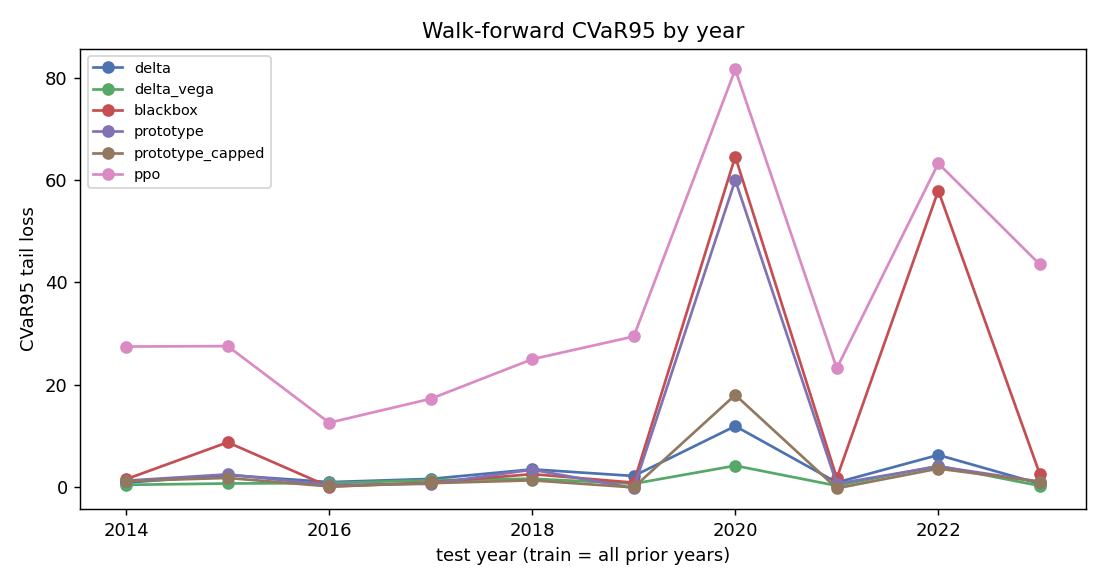
\includegraphics[width=\linewidth]{walkforward_cvar.png}
  \caption{Walk-forward $\mathrm{CVaR}_{95}$ by test year (real SPY). The deep
  hedgers blow up (note PPO across all years and the MLP in 2020/2022); the
  volatility-capped prototype repairs most of the prototype's 2020 failure.}
  \label{fig:walkforward}
\end{figure}

\subsection{Ablations}

\begin{table}[t]
\centering
\caption{Ablations (synthetic). The CVaR term is essential: dropping it explodes
the tail.}
\label{tab:ablation}
\small
\begin{tabular}{lrrr}
\toprule
variant & $\mathrm{CVaR}_{95}$ & $\mathrm{CVaR}_{99}$ & mean \\
\midrule
$K=4$                 & 1.38 & 1.75 & $-0.11$ \\
$K=8$ (default)       & \textbf{1.30} & 1.76 & $+0.03$ \\
$K=16$                & 1.64 & 2.53 & $+0.14$ \\
$K=32$                & 1.84 & 2.67 & $+0.24$ \\
features = greeks-only  & 1.34 & 1.75 & $-0.13$ \\
features = surface-only & 1.60 & 1.96 & $-0.12$ \\
objective = mean-only   & \textbf{42.36} & 58.78 & $+1.15$ \\
no transaction costs    & 1.43 & 1.97 & $+0.20$ \\
\bottomrule
\end{tabular}
\end{table}

Table~\ref{tab:ablation} isolates each ingredient. The prototype count has a
sweet spot at $K=8$ (too few underfits, too many overfits). The full feature set
beats greeks-only and surface-only, quantifying the value of combining surface
shape with Greeks. Critically, replacing the CVaR objective with a mean-only
objective inflates $\mathrm{CVaR}_{95}$ from $1.30$ to $\mathbf{42.4}$
(synthetic) and to $\mathbf{87.6}$ on real data---the risk objective is what
buys the tail control.

%% =====================================================================
\section{Interpretability}
\label{sec:interpretability}

\begin{figure}[t]
  \centering
  
\includegraphics[width=\linewidth]{hero_surface_vocabulary.png}
  \caption{The model's learned \emph{regime vocabulary}: each prototype reconstructs
  to a concrete implied-volatility surface. A low-level, gently sloped surface (left)
  is the calm-regime prototype; a high-level, steep surface (right) is the stressed
  one. This is the object the hedge keys on, and the explanation \emph{is} the decision.}
  \label{fig:proto_surf}
\end{figure}

\begin{figure}[t]
  \centering
  
\includegraphics[width=\linewidth]{hero_regime_map.png}
  \caption{Market-state regime map (PCA of the standardised state on the SPY test set):
  calm and stressed states separate, and the learned prototypes (stars) anchor distinct
  regions of the space.}
  \label{fig:regimemap}
\end{figure}

A primary benefit of the prototype head is auditability. Each prototype
reconstructs to a concrete IV surface (Figure~\ref{fig:proto_surf}) and a
readable hedge action, and the prototypes tile the market-state space into calm and
stressed regions (Figure~\ref{fig:regimemap}). A single stressed episode can be read
end to end (Figure~\ref{fig:anatomy}): the surface it faces, which prototypes activate,
the small bounded residual placed on the delta--vega hedge, and the resulting P\&L.
On real data the catalogue maps prototypes to historical
regimes: a high-level, steep-skew prototype activates predominantly in stressed
windows (high stress fraction), while low-level, gently sloped prototypes
dominate calm periods. The activation timeline
(Figure~\ref{fig:real_activation}) shows which regime drives the hedge through
the test period. Every action is attributable
to named market regimes. We note an honest caveat: on the long real sample the
learned residual is small (mean activation entropy ${\approx}0.11$), so the
prototype largely \emph{reproduces} delta--vega rather than learning sharply
distinct regime actions; the rich, differentiated behaviour is clearest on the
synthetic market, which motivates a regime-\emph{diagnostic} reading of the model
on real data.

\begin{figure}[t]
  \centering
  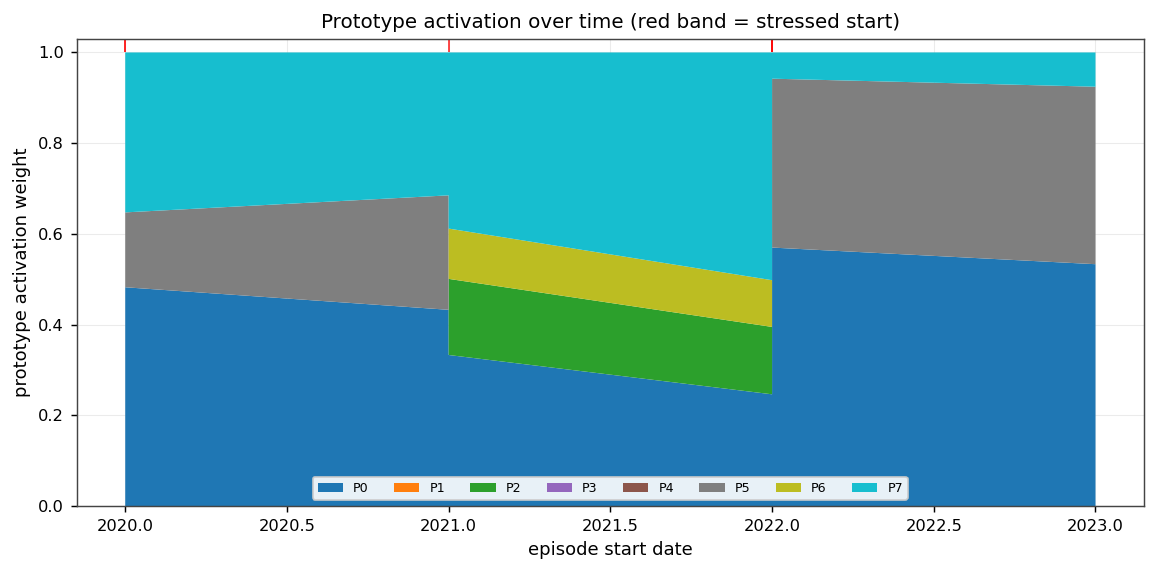
\includegraphics[width=\linewidth]{real_activation_timeline.png}
  \caption{Prototype activation over the real SPY test period: which volatility
  regime drives the hedge, when.}
  \label{fig:real_activation}
\end{figure}

\begin{figure}[t]
  \centering
  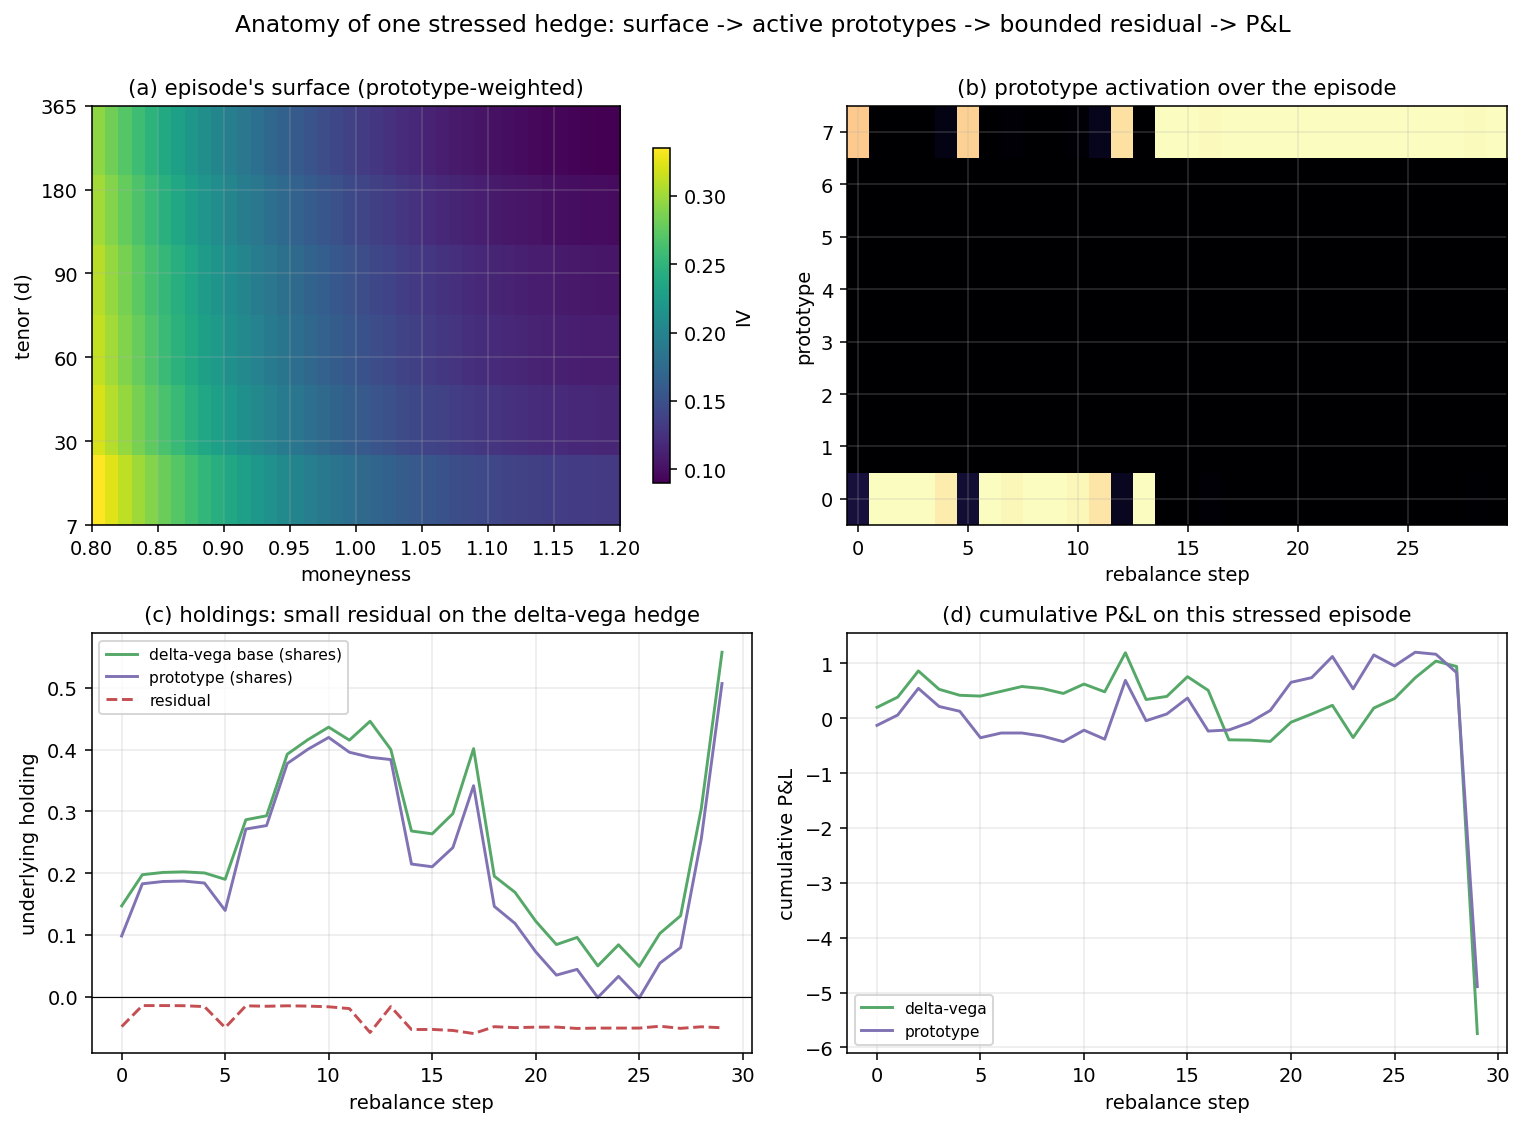
\includegraphics[width=\linewidth]{hero_hedge_anatomy.png}
  \caption{Anatomy of one stressed hedge (worst delta--vega episode on the SPY test
  set): (a) the prototype-weighted IV surface, (b) prototype activation over the
  episode, (c) the small bounded residual placed on the delta--vega holdings, and
  (d) cumulative P\&L versus delta--vega. The decision is fully traceable.}
  \label{fig:anatomy}
\end{figure}

%% =====================================================================
\section{Limitations}
\label{sec:limitations}

The tail-weighted prototype \emph{ties} delta--vega out-of-sample rather than beating
it significantly: the favourable cross-market estimate ($p=0.079$) is a robust tie, not
a proven win, and on QQQ a well-tuned MLP retains a better point estimate (though it is
seed-unstable). The honest claim is parity with the strongest classical baseline across
two markets, plus dominance over every deep-RL hedger and unique stability---not raw
outperformance of delta--vega. The fix was found by a search with validation-only
selection; we report the full grid, and note that naive validation-excess selection
\emph{overfits} under regime shift (a cautionary result), so the tail-weighting claim
rests on the pre-registered hypothesis confirmed on both markets' held-out tests. Over
the long horizon the residual is conservative (it stays near delta--vega; activation
entropy ${\approx}0.11$), so the edge is in robustness and drawdown rather than dramatic
regime-switching trades, and interpretability is most vivid on synthetic data. The
deep-RL comparators use default stable-baselines3 MLP policies at a fixed timestep
budget; a heavily tuned recurrent deep hedger might be less fragile, though the
overfitting finding holds across two markets and five seeds. The study covers two
underlyings (SPY, QQQ) but a single liability (one 30d ATM option) and a daily
rebalance; the underlying hedge leg uses the ETF (tradable), an SPX study would need a
futures proxy; costs are a proportional half-spread with no market-impact or borrow
modelling; and path-dependent payoffs would require a richer state.

%% =====================================================================
\section{Conclusion and Future Work}
\label{sec:conclusion}

A small, auditable set of volatility-surface prototypes delivers hedging that is
\emph{fully interpretable} and, across two real markets (SPY, QQQ), \emph{matches the
strongest classical baseline} (delta--vega) on the tail while being \emph{markedly more
robust than every learned black-box and deep-RL hedger} (MLP, PPO, SAC), which overfit
in-sample drift and blow up out-of-sample. Crucially, the cross-market parity did not
come for free: a naive anchored residual lost on QQQ, and only a \emph{tail-weighted
objective}---identified by a pre-registered search with validation-only selection and
confirmed on both markets' held-out tests---made the robustness transfer. The
defensible headline is that a constrained, interpretable policy can be as safe as
classical hedging and far safer than unconstrained deep hedging: transparency and
tail-risk control need not be traded against one another. The CVaR objective (and its
tail weighting), residual anchoring, and the volatility-scaled cap are the ingredients
that make this work.

Future work proceeds along three axes. \emph{Beyond parity:} recover a significant
edge over delta--vega via a regime-diagnostic residual or richer surface dynamics.
\emph{Empirical breadth:} extend to SPX with a futures delta proxy, to more underlyings
and path-dependent payoffs. \emph{Comparative evaluation:} benchmark against heavily
tuned recurrent deep hedgers under more realistic dynamics, and engage practitioners to
assess the prototype catalogue as a decision-support artefact.

%% =====================================================================
\begin{acks}
Artefacts, figures and tables in this paper are produced by the open pipeline in
the project repository and are reproducible end to end.
\end{acks}

\bibliographystyle{ACM-Reference-Format}
\bibliography{references}

\end{document}
